Here is the TikZ LaTeX code for generating the 1-neighborhoods of the black vertex in the three grids you described:

```latex
\documentclass{standalone}
\usepackage{tikz}

\begin{document}

% Define colors
\definecolor{black}{rgb}{0,0,0}
\definecolor{white}{rgb}{1,1,1}

% Draw the square grid
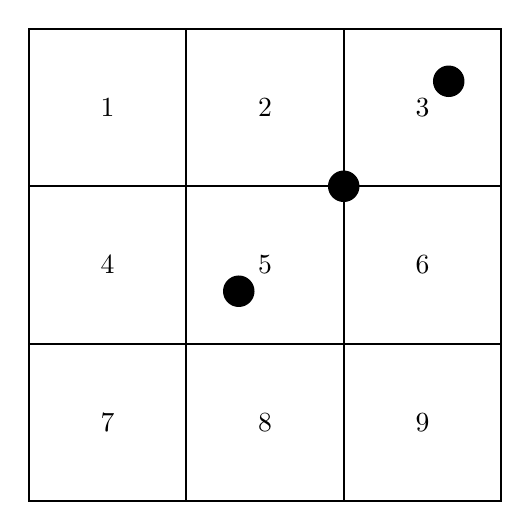
\begin{tikzpicture}[scale=2]
    \draw[thick] (0,0) rectangle (3,3);
    \draw[thick] (1,0) -- (1,3);
    \draw[thick] (2,0) -- (2,3);
    \draw[thick] (0,1) -- (3,1);
    \draw[thick] (0,2) -- (3,2);

    % Label the vertices
    \node at (0.5,2.5) {1};
    \node at (1.5,2.5) {2};
    \node at (2.5,2.5) {3};
    \node at (0.5,1.5) {4};
    \node at (1.5,1.5) {5};
    \node at (2.5,1.5) {6};
    \node at (0.5,0.5) {7};
    \node at (1.5,0.5) {8};
    \node at (2.5,0.5) {9};

    % Highlight the 1-neighborhood of the black vertex (let's say it's vertex 5)
    \foreach \x in {4,6,8} {
        \fill[black] (\x/3,\x/3) circle (0.1);
    }
\end{tikzpicture}

% Draw the king grid
\begin{tikzpicture}[scale=2]
    \draw[thick] (0,0) rectangle (3,3);
    \draw[thick] (1,0) -- (1,3);
    \draw[thick] (2,0) -- (2,3);
    \draw[thick] (0,1) -- (3,1);
    \draw[thick] (0,2) -- (